% Straight up stealing preamble from Eli Holmes 
%%%%%%%%%%%%%%%%%%%%%%%%%%%%%%%%%%%%%%START PREAMBLE THAT IS THE SAME FOR ALL EXAMPLES
\documentclass{article}

%Required: You must have these
\usepackage{Sweave}
\usepackage{graphicx}
\usepackage{tabularx}
\usepackage{hyperref}
\usepackage{natbib}
%\usepackage[backend=bibtex]{biblatex}
%Strongly recommended
  %put your figures in one place
%\SweaveOpts{prefix.string=figures/, eps=FALSE} 
%you'll want these for pretty captioning
\usepackage[small]{caption}

\setkeys{Gin}{width=0.8\textwidth}  %make the figs 50 perc textwidth
\setlength{\captionmargin}{30pt}
\setlength{\abovecaptionskip}{0pt}
\setlength{\belowcaptionskip}{10pt}
% manual for caption  http://www.dd.chalmers.se/latex/Docs/PDF/caption.pdf

%Optional: I like to muck with my margins and spacing in ways that LaTeX frowns on
%Here's how to do that
 \topmargin -1.5cm        
 \oddsidemargin -0.04cm   
 \evensidemargin -0.04cm  % same as oddsidemargin but for left-hand pages
 \textwidth 16.59cm
 \textheight 21.94cm 
 %\pagestyle{empty}       % Uncomment if don't want page numbers
 \parskip 7.2pt           % sets spacing between paragraphs
 %\renewcommand{\baselinestretch}{1.5} 	% Uncomment for 1.5 spacing between lines
\parindent 0pt% sets leading space for paragraphs
\usepackage{setspace}
%\doublespacing

%Optional: I like fancy headers
\usepackage{fancyhdr}
\pagestyle{fancy}
\fancyhead[LO]{How do climate change experiments actually change climate}
\fancyhead[RO]{2016}
 
%%%%%%%%%%%%%%%%%%%%%%%%%%%%%%%%%%%%%%END PREAMBLE THAT IS THE SAME FOR ALL EXAMPLES

%Start of the document
\begin{document}

%\SweaveOpts{concordance=TRUE}
 \bibliographystyle{/Users/aileneettinger/citations/Bibtex/styles/nature.bst}
\title{How do climate change experiments actually change climate?} % Paper 1/Large group paper from Reconciling Experimental and Observational Approaches for Climate Change Impacts

\author{A.K. Ettinger,I. Chuine, B. Cook, J. Dukes, A.M. Ellison, M.R. Johnston, A.M. Panetta,\\ C. Rollinson, Y. Vitasse, E. Wolkovich}
%\date{\today}
\maketitle  %put the fancy title on
%\tableofcontents      %add a table of contents
%\clearpage
%%%%%%%%%%%%%%%%%%%%%%%%%%%%%%%%%%%%%%%%%%%%%%%%%%%


\section* {Supplemental Materials}

\par To realize the forecasting potential of climate change experiments, a nuanced understanding of how climate change experiments actually alter climate is critical. Here, we use  plot-level daily  microclimate  data  from  12 climate  change  experiments  that  manipulate temperature and precipitation to demonstrate the direct and indirect ways in which environmental conditions are altered  by active  warming technologies. We then highlight the challenges associated with quantifying and interpreting biological responses to these climate manipulations, and using these interpretations to forecast  more widespread responses to contemporary climate change. Finally,  we use findings from our synthesis to make recommendations for future  climate  change experiments.  We focus on in situ active warming  manipulations, because recent analyses indicate that active warming methods are the most controlled, consistent, and ``true to climate change predictions" \citep{kimball2005,kimball2008,aronson2009,wolkovich2012}. The data we use were collected between 1991 and 2014 from North American and European climate change experiments and  have been merged into a new, publicly  available  Climate from Climate Change Experiments (C3E) database (see Supplemental Materials  for details). 

\par We carried out a full literature review to identify all active field warming experiments then obtained daily (or sub-daily) climate data from as many as possible (we obtained data for 12/XX total identified experiments. We are thus able to show, for the first time, the complex ways that climate is altered by active warming treatments, both directly and indirectly. 

\bibliography{/Users/aileneettinger/citations/Bibtex/mylibrary}
\clearpage
\section* {Supplemental Tables}

% EMW all tables should go into supp and give the results parenthetically in main text (sweavedemo has an example of how to do this). Also be SURE TO GIVE ERROR DF throughout. 

%Yann:I know it is the direct output but don't forget for a cleaner version to just write < 0.001, write integer numbers for df and round the Chisq to keep less numbers
% latex table generated in R 3.2.4 by xtable 1.8-2 package
% Thu Feb 16 10:15:56 2017
\begin{table}[ht]
\centering
\begin{tabular}{lrrr}
  \hline
 & Chisq & Df & Pr($>$Chisq) \\ 
  \hline
(Intercept) & 153.303 & 1.000 & 0.000 \\ 
  temptreat & 463.345 & 3.000 & 0.000 \\ 
  block & 3.955 & 2.000 & 0.138 \\ 
  temptreat:block & 44.881 & 6.000 & 0.000 \\ 
   \hline
\end{tabular}
\caption{Effects of warming vary by block, as summarized by a linear mixed effects model of mean soil temperatures, with year and site as nested random effects} 
\end{table}
% latex table generated in R 3.2.4 by xtable 1.8-2 package
% Thu Feb 16 10:15:56 2017
\begin{table}[ht]
\centering
\begin{tabular}{lrrr}
  \hline
 & Chisq & Df & Pr($>$Chisq) \\ 
  \hline
(Intercept) & 1455.294 & 1.000 & 0.000 \\ 
  temptreat & 126.093 & 3.000 & 0.000 \\ 
  year & 16.676 & 1.000 & 0.000 \\ 
  temptreat:year & 61.646 & 3.000 & 0.000 \\ 
   \hline
\end{tabular}
\caption{Effects of warming vary by year, as summarized by a linear mixed effects model of mean soil temperatures, with year and site as nested random effect} 
\end{table}\par The below are all tables related to the sham and ambient comparisons. i want to include more information in the tables, probably (random effects- intercepts, and variance), and most will be in the supplemental (perhaps just the mean soil and air in the main text?)
.
\par 
% latex table generated in R 3.2.4 by xtable 1.8-2 package
% Thu Feb 16 10:16:00 2017
\begin{table}[ht]
\centering
\begin{tabular}{rrrr}
  \hline
 & Estimate & Std. Error & t value \\ 
  \hline
(Intercept) & 12.691 & 1.648 & 7.699 \\ 
  controltypeambient & -0.311 & 0.092 & -3.380 \\ 
   \hline
\end{tabular}
\caption{Summary of linear mixed effects model testing difference in mean air temperatures of structural controls compared with ambient controls (i.e.with no control chambers or warming infrastructure in place). The model included a fixed effect of control type and an intercept-only random effect of studysite to account for study and measurement, as well as environmental, differences.} 
\end{table}
\par
% latex table generated in R 3.2.4 by xtable 1.8-2 package
% Thu Feb 16 10:16:00 2017
\begin{table}[ht]
\centering
\begin{tabular}{rrrr}
  \hline
 & Estimate & Std. Error & t value \\ 
  \hline
(Intercept) & 11.315 & 1.373 & 8.243 \\ 
  controltypeambient & 0.450 & 0.067 & 6.682 \\ 
   \hline
\end{tabular}
\caption{Summary of linear mixed effects model testing difference in mean soil temperature (at the shallowest depth measured) of structural controls compared with ambient controls. The model included a fixed effect of control type and an intercept-only random effect of studysite to account for study and measurement, as well as environmental, differences.} 
\end{table}
\par
% latex table generated in R 3.2.4 by xtable 1.8-2 package
% Thu Feb 16 10:16:00 2017
\begin{table}[ht]
\centering
\begin{tabular}{rrrr}
  \hline
 & Estimate & Std. Error & t value \\ 
  \hline
(Intercept) & 7.178 & 1.397 & 5.138 \\ 
  controltypeambient & -0.343 & 0.092 & -3.744 \\ 
   \hline
\end{tabular}
\caption{Summary of linear mixed effects model testing difference in minimum air temperatures of structural controls compared with ambient controls (i.e.with no control chambers or warming infrastructure in place). The model included a fixed effect of control type and an intercept-only random effect of studysite to account for study and measurement, as well as environmental, differences.} 
\end{table}\par
% latex table generated in R 3.2.4 by xtable 1.8-2 package
% Thu Feb 16 10:16:00 2017
\begin{table}[ht]
\centering
\begin{tabular}{rrrr}
  \hline
 & Estimate & Std. Error & t value \\ 
  \hline
(Intercept) & 10.503 & 1.343 & 7.823 \\ 
  controltypeambient & 0.386 & 0.068 & 5.693 \\ 
   \hline
\end{tabular}
\caption{Summary of linear mixed effects model testing difference in minimum soil temperature (at the shallowest depth measured) of structural controls compared with ambient controls. The model included a fixed effect of control type and an intercept-only random effect of studysite to account for study and measurement, as well as environmental, differences.} 
\end{table} 
% latex table generated in R 3.2.4 by xtable 1.8-2 package
% Thu Feb 16 10:16:00 2017
\begin{table}[ht]
\centering
\begin{tabular}{rrrr}
  \hline
 & Estimate & Std. Error & t value \\ 
  \hline
(Intercept) & 18.204 & 1.915 & 9.504 \\ 
  controltypeambient & -0.278 & 0.097 & -2.851 \\ 
   \hline
\end{tabular}
\caption{Summary of linear mixed effects model testing difference in maximum air temperatures of structural controls compared with ambient controls (i.e.with no control chambers or warming infrastructure in place). The model included a fixed effect of control type and an intercept-only random effect of studysite to account for study and measurement, as well as environmental, differences.} 
\end{table}
% latex table generated in R 3.2.4 by xtable 1.8-2 package
% Thu Feb 16 10:16:00 2017
\begin{table}[ht]
\centering
\begin{tabular}{rrrr}
  \hline
 & Estimate & Std. Error & t value \\ 
  \hline
(Intercept) & 13.602 & 1.674 & 8.125 \\ 
  controltypeambient & 0.588 & 0.076 & 7.770 \\ 
   \hline
\end{tabular}
\caption{Summary of linear mixed effects model testing difference in maximum soil temperature (at the shallowest depth measured) of structural controls compared with ambient controls. The model included a fixed effect of control type and an intercept-only random effect of studysite to account for study and measurement, as well as environmental, differences.} 
\end{table}

\clearpage
\section*{Supplemental Materials}
\subsection*{Description of database}
Search terms used and criteria for selecting the 12 studies that we ended up with. Climate variables included, and where database and metadata are housed.
\subsection*{Supplemental Methods}
\par\textit{Statistical methods}
\par Need description of block and year analyses (see Tables 1 and 2) 
To account for differences in the type of warming and other unmeasured site/study differences (e.g. forced air for Ellison and Marchin; heating cables for Farnsworth and ??), we fit linear mixed effects models with random effect of study-site. Response variables were daily soil or air temperature (models with daily  mean, minimum, and maximum were all fit) and , and the explanatory variable was control type (infrastructure or ambient). We used a random intercepts structure, so that the mean temperature was allowed to vary across study-sites. We fit models across the entire year, as well as separate models for each month to examine if effects varied seasonally.
\subsection*{Random stuff moved out of the main text}
We also found higher coefficients of variation in air temperatures in actively warmed plots, compared with controls at the same sites in the same years. This was true for both minimum and maximum air temperatures (Figure \ref{fig:cv})


\begin{figure}[p]
\centering
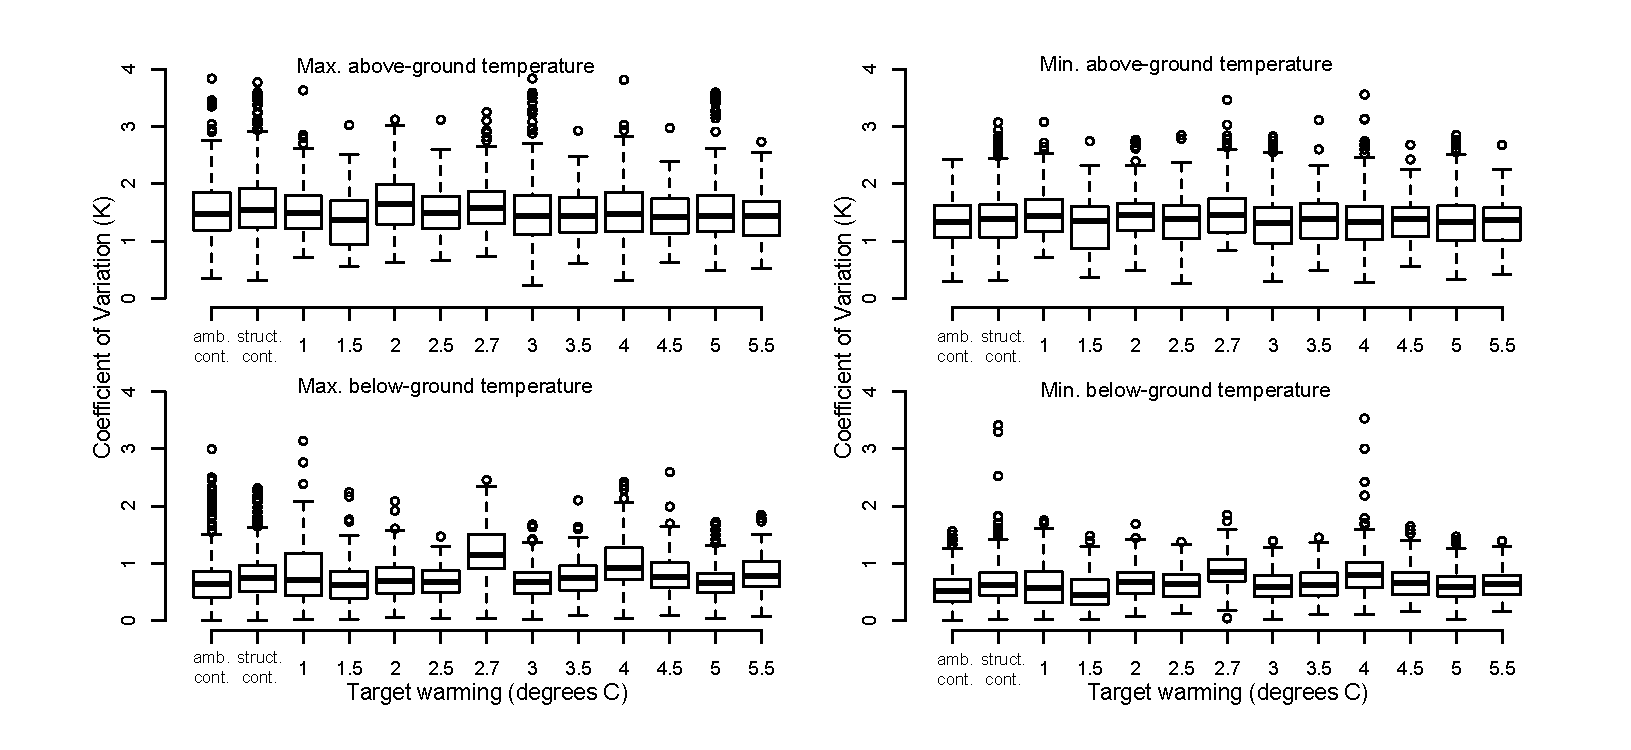
\includegraphics{../Analyses/figures/DRAFT_CVBytreatment.pdf} 
\caption{Ambient controls have reduced variation, compared with structural controls and nearly all warming treatments. I'm not happy with this figure- I've tried so many different ways of showing the (small but) significant differences in temperature range/variance among ambient controls, structural controls and warming treatments, in addition to the statistical analyses described in the text and supplement. Question for everyone (Lizzie/Ben/Miriam/Ann Marie/Aaron/Yann/Isabelle/Jeff/Christy): I need help with ideas for other ways to show this, or thoughts on if the point should be dropped, since the differences are minor and hard to see.} %Aaron: why not just plot variance? From this figure, the reader has to infer variance. This figure also collapses time into a single box. What about illustrating temporal variance (i.e., the time-series)? Which is what the next figure does very effectively. Yann: or maybe subtract the standard deviation of the ambient control from the structural control and finally all warming treatments?
%Christy: I think I’m in favor of dropping this figure… I think part of the problem is that there are just a ton of warming levels and your combining across a bunch of different experiments and it’s not clear what is different.%Jeff: I don’t think I understand what’s going on with this figure.  I am not sure what the individual data points are.  Something like Yann’s suggestion sounds reasonable, though.  But a more descriptive legend would really help.   Do we really want to look at some longer-term CV, or do we want something more like DTR?
% EW: Fig 2 should be in the supplement and I had some ideas to make it look better.

 \label{fig:cv}
 \end{figure}
%%%%%%%%%%%%%%%%%%%%%%%%%%%%%%%%%%%%%%%%
\end{document}
%%%%%%%%%%%%%%%%%%%%%%%%%%%%%%%%%%%%%%%%
